\documentclass[tikz, border=10pt]{standalone}
\usetikzlibrary{automata, positioning, arrows}

\begin{document}

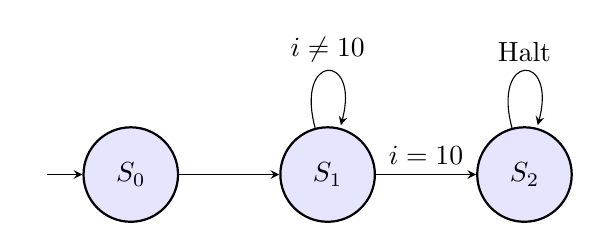
\begin{tikzpicture}[
    ->, >=stealth, auto, node distance=2.5cm,
    every state/.style={thick, fill=blue!10, minimum size=1.2cm},
    initial text=$ $
]

    \node[state, initial] (S0) {$S_0$};
    \node[state, right of=S0] (S1) {$S_1$};
    \node[state, right of=S1] (S2) {$S_2$};

    \path   (S0) edge node {} (S1)
            (S1) edge [loop above] node {$i \neq 10$} (S1)
            (S1) edge node {$i = 10$} (S2)
            (S2) edge [loop above] node {Halt} (S2);

\end{tikzpicture}

\end{document}
